\section{Experimental Results}
\label{sec:experiments}

\subsection{Experimental Setup}


In this milestone report, we show experimental results when we apply KNN method to sequences of CPU usage measurements data.
We used Samsung Galaxy S device on which Android 2.3 Gingerbread is running, and Netflix application was used for collecting CPU usage statistics.
10 movies are selected from \term{Popular on Netflix} section of Netflix website and selected movies are shown in Table \ref{tab:movies}.
CPU statistics of selected movies were captured by recording CPU statistics in 5-second interval using the native UNIX command, \term{top}, while playing the first 30 minutes of each movie. 
The measurement was repeated 5 times for each movie.
Measurement results of two selected movies are previously shown in Figure \ref{fig:preliminaries}.

\begin{table}[h!]
\vspace{-5mm}
\begin{center}
\begin{tabular}{|c|l|c|l|}
\hline
ID & Movie Title & ID & Movie Title \\ 
\hline
1 & Transformers: Dark of the Moon 		& 2 & Thor \\
3 & Hachi: A Dog's Tale 			& 4 & The True Story of Puss 'n Boots \\
5 & Wallace \& Gromit: Loaf and Death 	& 6 & Super 8 \\
7 & Mean Girls 2 				& 8 & Captain America \\
9 & Snatch 					& 10 & No Strings Attached \\
\hline
\end{tabular}
\end{center}
\caption{Selected Movies}
\label{tab:movies}
\end{table}
\vspace{-15mm}

\subsection{KNN Experiment Results}

For each movie, one of five CPU usage sequence is selected as test data and the rest four sequences are considered as training data set. 
The length of subsequence varying from 60 seconds to 360 seconds is set and each test and training data is divided based on the subsequence length as described in \ref{sec:knn}.
When dividing sequence data, we adopt a concept of sliding window which moves by 1 step size.
Each data sequence consists of $360$ measurement points, and therefore $(360 - subsequence\_length + 1)$ subsequences are generated from the data sequence. 

After building up test data set and training data set by generating subsequences, we apply KNN method in order to classify each subsequence of test data based on training data set. 
In this experiment, $k$ value is set to 3 for the simplicity.
The accuracy of classification according to the length of subsequence is shown in Figure \ref{fig:experiment_knn}.
The accuracy is low as 46$\%$ when subsequence length is set to 60-second.
However, the accuracy increases up to 88$\%$ when subsequence is set to 180-second.
The experimental result shows that given 10 movies and CPU usage statistics of 150 seconds, our side channel attack correctly predicts which movie a user is watching at the accuracy of higher than 80$\%$.

\begin{figure}[!ht]
\centering
\includegraphics[scale=0.50]{Figures/experiment_knn}
\caption{KNN Classification Accuracy}
\label{fig:experiment_knn}
\vspace{-5mm}
\end{figure}






%%%%%%%%%%%%%%%%%%%%%%%%%%%%%%%%%%%%%%%%%%%%%%%%%%%%%%%%%%%%%

\begin{comment}
For the project milestone, we collected CPU statistics for 10 movies. 
Each statistic is captured by recording CPU statistics using the native UNIX command, Top, while playing 30-minute long video sequence. 
Video sequences and a query sequence are measured in 1 second interval which is the most fine-grained time interval in the Top command.
\end{comment}


\begin{comment}
\subsection{Overview}
In this section, we describe 1) how CPU statistics for movies are collected, 2) how the collected raw data are processed to be useful in building up datasets and 3) how the processed data are stored in the datasets.

For the project milestone, we collected CPU statistics for 10 movies. Each statistic is captured by recording CPU statistics using the native UNIX command, Top, while playing 30-minute long video sequence. Video sequences and a query sequence are measured in 1 second interval which is the most fine-grained time interval in the Top command. To efficiently match a subsequence, a query sequence, to the collected video sequence in the dataset, we converted the time series datasets (i.e. the video sequence and the query sequence) into datasets in spatial space. To build-up the datasets largely consists of two jobs: pre-processing raw data sequences and storing the processed sequences into a data structure.
\begin{figure}[!ht]
\centering
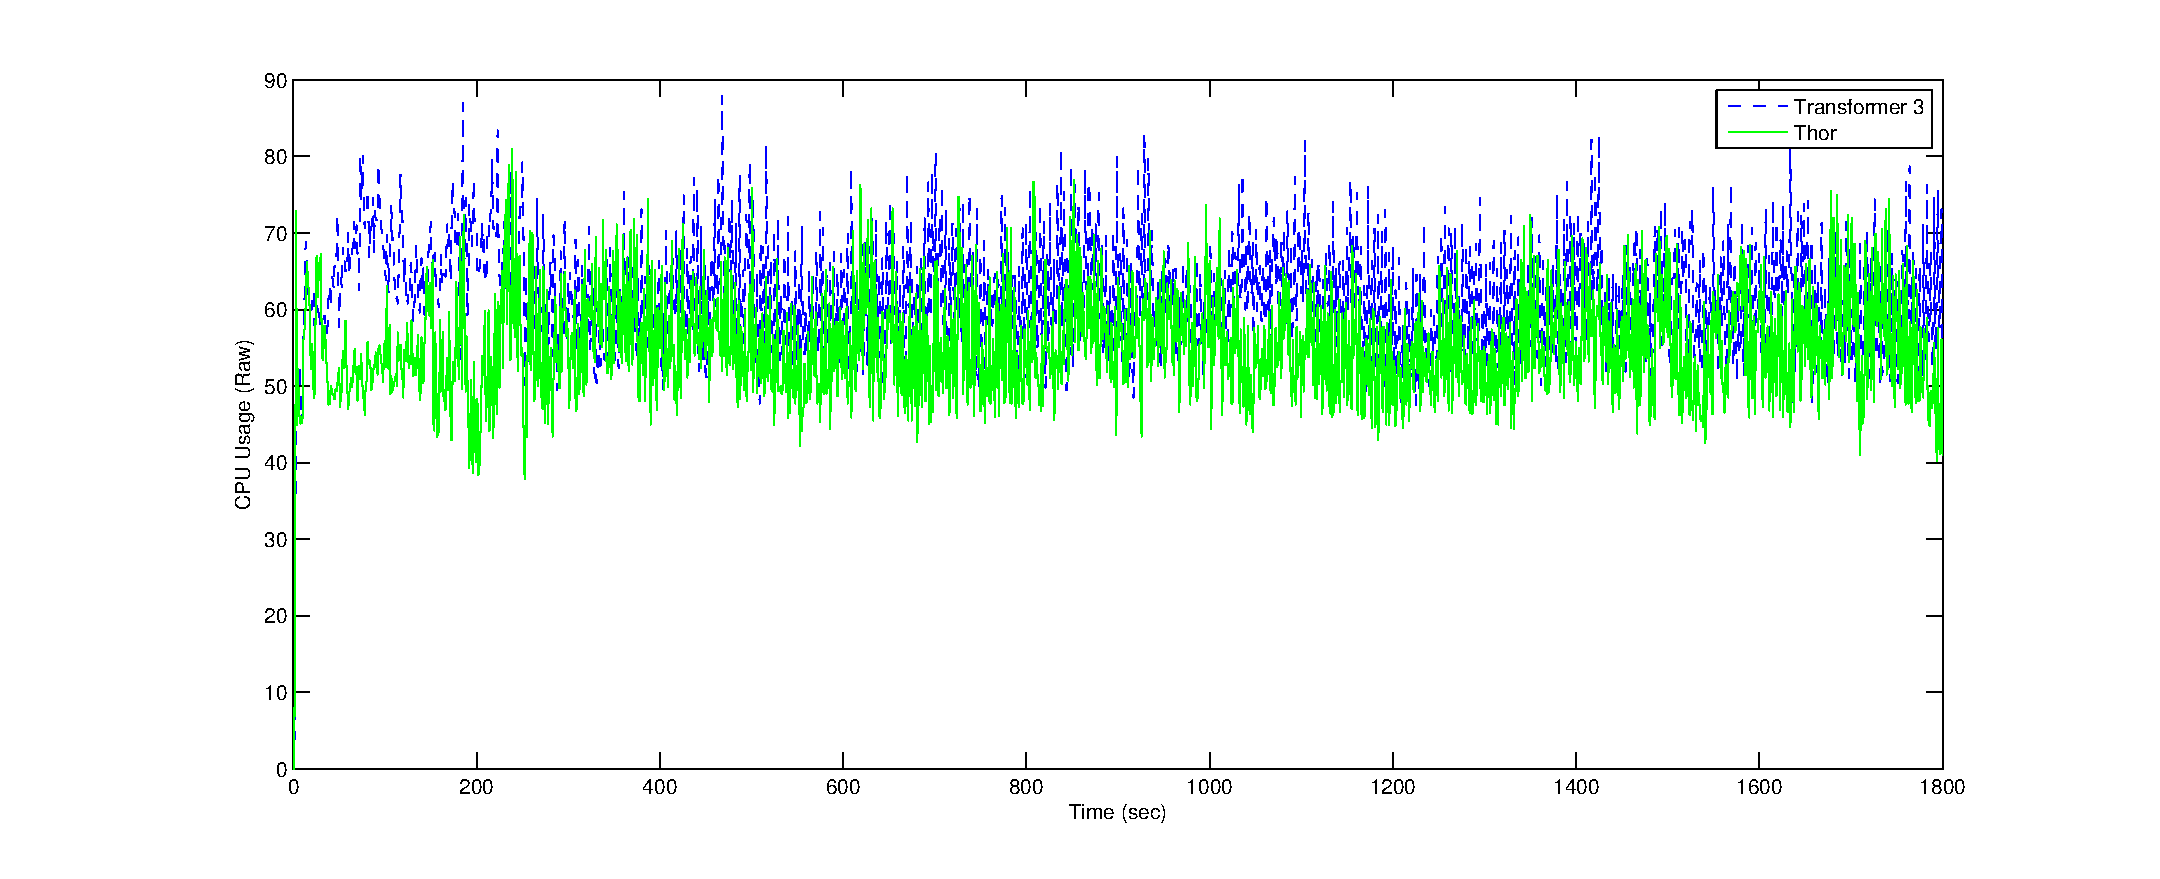
\includegraphics[scale=0.35]{Figures/RAW_TF_Thor}
\caption{XXX}
\end{figure}

\begin{figure}[!ht]

	\subfigure[RAW] {
		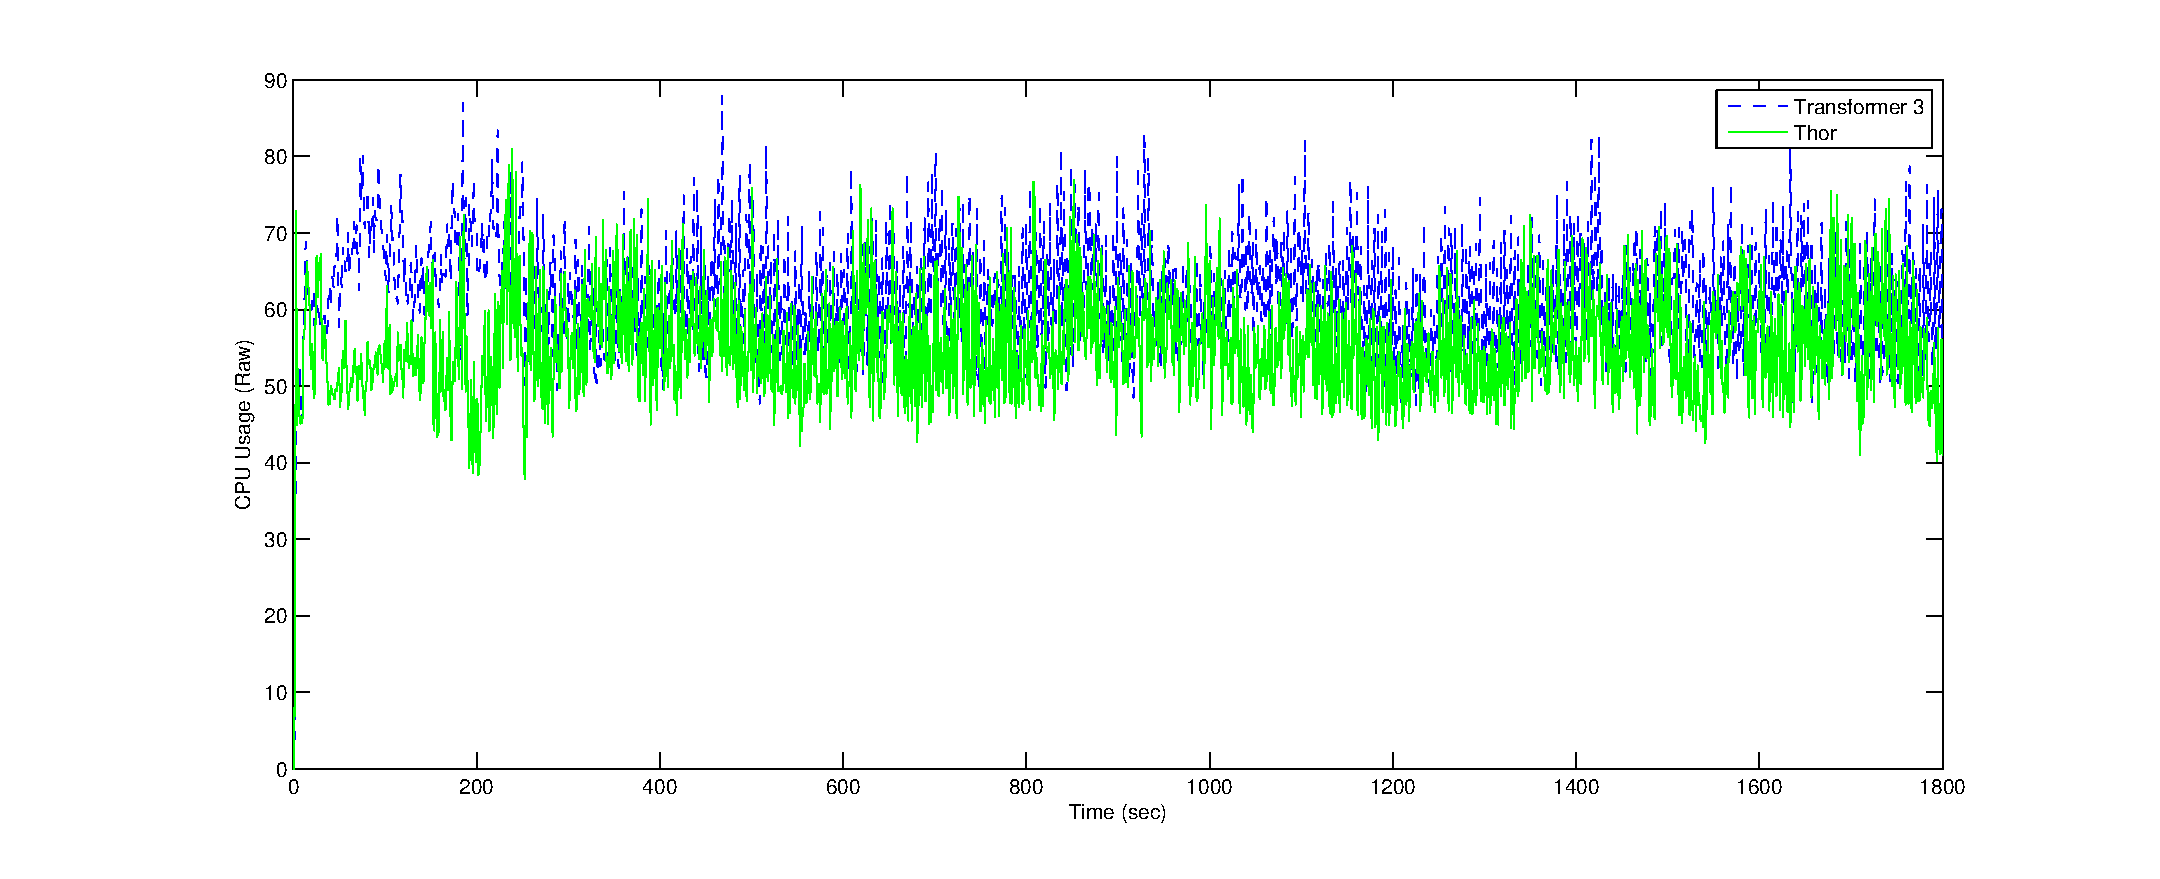
\includegraphics[scale=0.5]{Figures/RAW_TF_Thor.eps}
		\label{fig:preliminary_thor}
	}
	\subfigure[SMTH_TF_Thor] {
		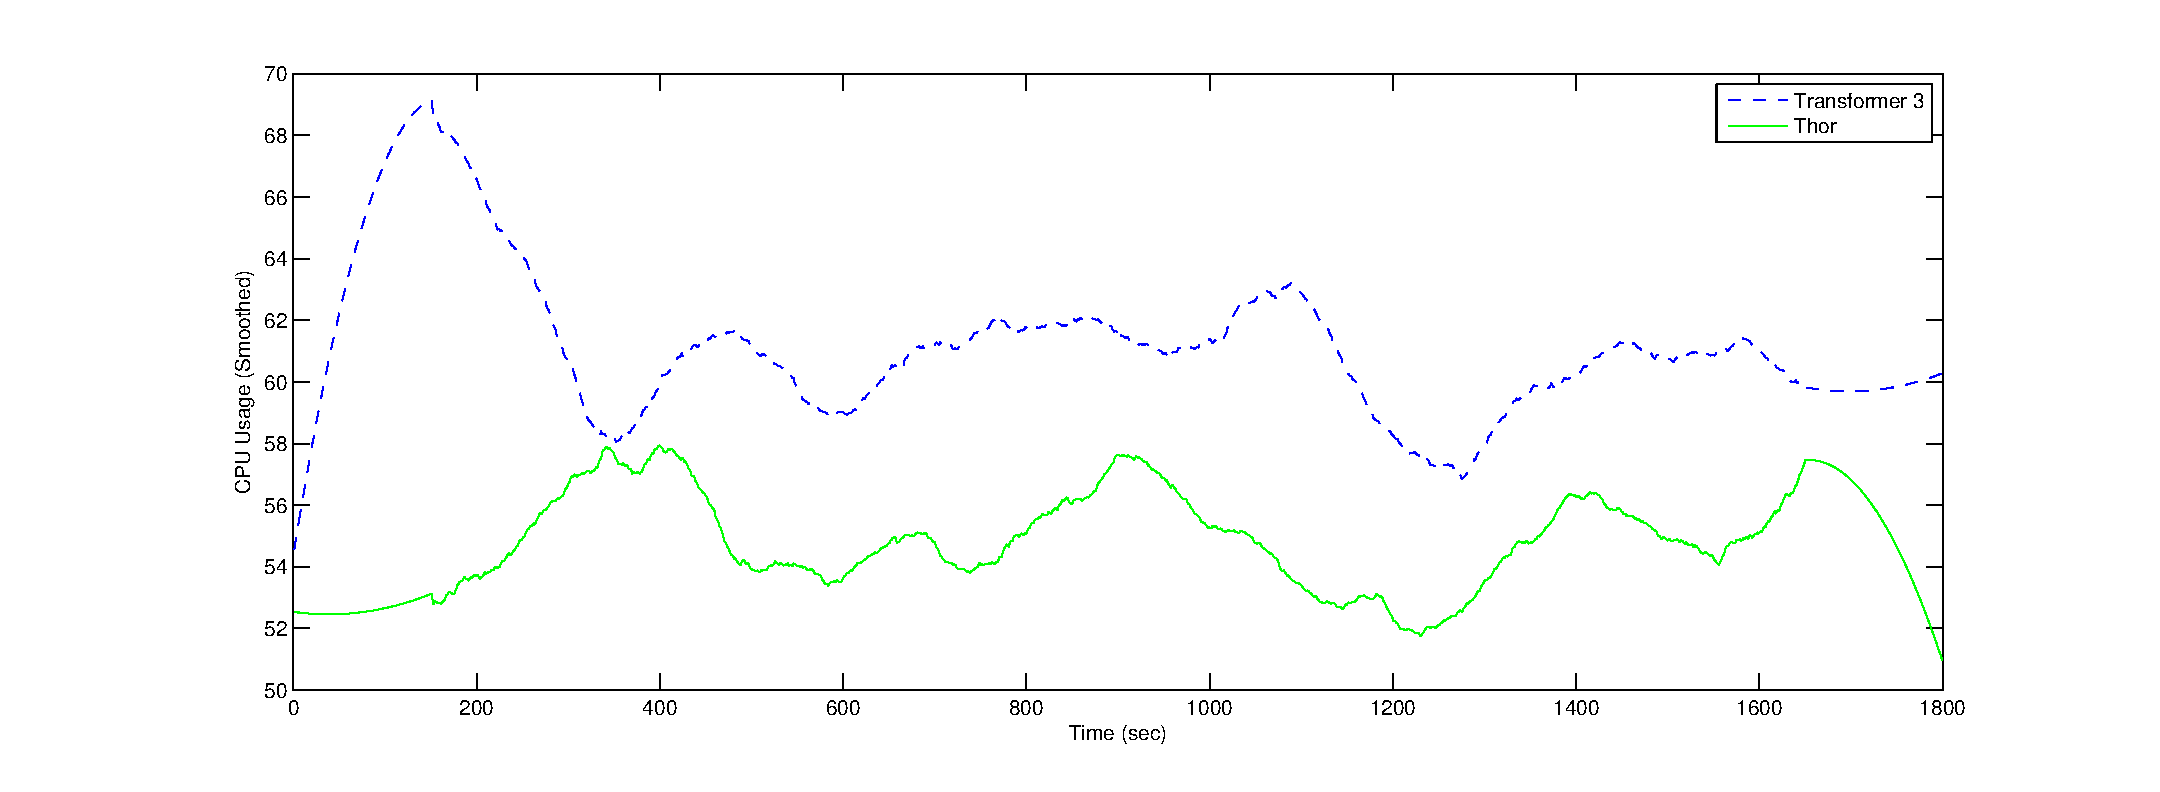
\includegraphics[scale=0.5]{Figures/SMTH_TF_Thor.eps}
		\label{fig:preliminary_thor}
	}
	\caption{CPU Usage Measurements of two movies}
	\label{fig:preliminaries}
\end{figure}

\subsection{Pre-processing raw data sequences}
For the same movie title, we collected cpu statistics for five times under the same environment. To remove the noise in the raw data, we used the Savitzky-Golay smoothing filter which is commonly used to filter out noise in time series data \cite{SGfilter}. The SG filter averages n adjacent points to flatten noise while preserving features of the distribution. In the experiment, we set the window length as 300. After smoothing, five cpu statistic streams were averaged because each statistic has little different amplitudes. Before averaging, streams needed to be aligned and trimmed appropriately because the data collection was manually done by hands. We set the first stream of each movie as a reference to the other 4 streams, and performed cross-correlation to obtain a time-lag which gives a point where streams are most similar. Once the alignment was done, the amplitude of five streams are averaged, and the sequence with the averaged amplitude was stored in the datasets and was used as the reference sequence to a query sequence.

To convert the pre-processed sequences into data trails in the spatial domain, Discrete Fourier Transform (DFT) was applied to the pre-processed sequences. More specifically, a  DFT window of a specified length is used so that DFT could be applied to each subsequence within a video sequence from the starting index to the end index of the video sequence. At every DFT application to each subsequence, the first two Fourier coefficients were extracted, which made the time series data sequence to be 2-dimensional spatial data while preserving more than 80-percent of energy of the original sequence.

\subsection{Storing processed sequence into a data structure} 
For an efficient search operation, we decided to use R* tree\cite{Beckmann:1990}, which is a variant of R-tree. For first-approximation of spatial query, R* tree stores Minimum Bounding Rectangles (MBRs) that consist of multiple adjacent points in multi-dimensional space. In our project, the pre-processed video sequence can be depicted as a trail, which is a series of two-dimensional spatial points corresponding to the Fourier coefficients of each subsequence within the video sequence. On packing MBRs, the packing strategy used in \cite{Faloutsos:1994}\cite{Kamel:1993} is adopted to minimize the disk access cost in accessing a specific node in R* tree.

\end{comment}